\documentclass[12pt]{article}

\usepackage[margin=1in]{geometry}
\usepackage{amsmath}
\usepackage{hyperref}
\usepackage{graphicx}
\usepackage{booktabs}
\usepackage{enumitem}
\usepackage[T1]{fontenc}
\usepackage[utf8]{inputenc}

\hypersetup{
  colorlinks=true,
  linkcolor=blue,
  urlcolor=blue,
  citecolor=blue
}

\title{The Cosmic Microwave Background \& the Simons Observatory}
\author{Aashrita Mangu}
\date{}

\begin{document}

\maketitle

\textit{Please refer to my thesis for more information on the cosmic microwave background or the Simons Observatory experiment. Some of this text is adapted from there!}

\tableofcontents
\newpage

% ──────────────────────────────────────────────────────────────
\section{Introduction}

Much of experimental cosmology is geared towards answering the fundamental question of: \textit{How did the universe originate and evolve?} Over the past several decades, theoretical and experimental cosmology has advanced drastically and attempted to answer this and other prodigious questions with high precision. From Einstein's general relativity to modern highly sensitive observations of the cosmic microwave background, we have seen an evolution in testable theories that aim to answer fundamental questions about our universe.

% ──────────────────────────────────────────────────────────────
\section{Background}
\label{sec:background}

The most widely accepted theory of the history of the universe is the hot Big Bang model: our universe was once a hot, dense, opaque plasma that expanded and cooled over time. After about 380,000 years, the universe was cool enough to start forming neutral hydrogen, and photons were able to \textit{free stream} --- that is, there was enough room in the primordial soup for photons to not hit/scatter off of other particles floating around and break up elements. These photons (or light) that act as a faint glow that fills up the entire sky no matter where we look are known as the \textit{cosmic microwave background} (CMB). This radiation was emitted at \textit{recombination}, when the universe had cooled below $\sim$3000\,K (formation of neutral hydrogen). Since then, the CMB has redshifted (i.e.\ the wavelengths have stretched out with the expansion of the universe over billions of years) to a current temperature of $T_0 = 2.725$\,K.

The CMB appears nearly uniform across the sky, but contains anisotropies (small fluctuations) at the level 1 part in $10^5$. These tiny density fluctuations in the early universe are the seeds of large scale structure like galaxy clusters we see today. The CMB angular power spectrum (decomposing temperature fluctuations into multipole moments $\ell$) shows a series of acoustic peaks from sound waves in the primordial plasma that act as a cosmic ruler, precisely fixing cosmological parameters (Fig.~\ref{fig:planck_spectra}). Over time with efforts from both space-based satellites (e.g.\ the \textit{Wilkinson Microwave Anisotropy Probe} (WMAP) and \textit{Planck}) and ground-based observatories (e.g.\ the Atacama Cosmology Telescope (ACT), BICEP, South Pole Telescope (SPT), and POLARBEAR), anisotropies in CMB temperature and polarization have been mapped to great precision over many angular scales. Upcoming ground-based experiments such as Simons Observatory (SO) will hit unprecedented sensitivities and provide valuable cosmological information in the coming decades. They also provide the tools and technical readiness for space-based missions to reach sensitivities that are more difficult to achieve on earth with atmospheric interference.

\begin{figure}[htbp]
  \centering
  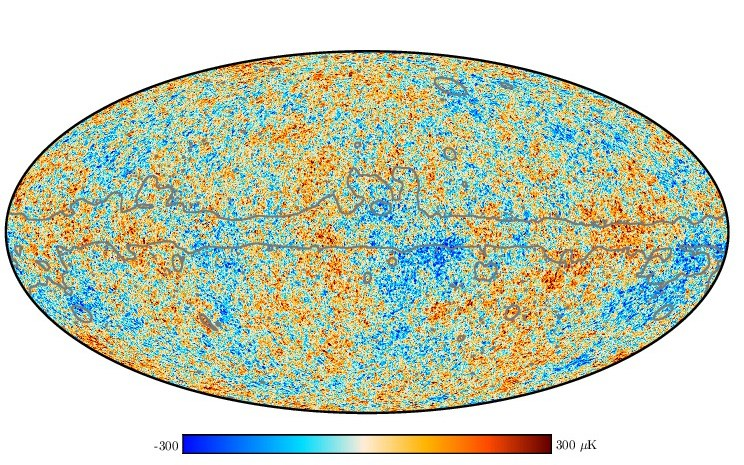
\includegraphics[width=0.85\textwidth]{img/img_03.jpg}
  \caption{\textbf{Planck 2018 SMICA CMB temperature map.} Full-sky CMB temperature anisotropies ($\Delta T / T \sim 10^{-5}$) from the Planck satellite. The grey line marks regions masked due to Galactic foreground emission. The rich structure encodes the initial conditions of the Universe and constrains all major cosmological parameters. \textit{Reproduced from Planck Collaboration (2020) (Fig.~22), CC-BY 4.0, \copyright\ ESA/Planck Collaboration.}}
  \label{fig:planck_map}
\end{figure}

\begin{figure}[htbp]
  \centering
  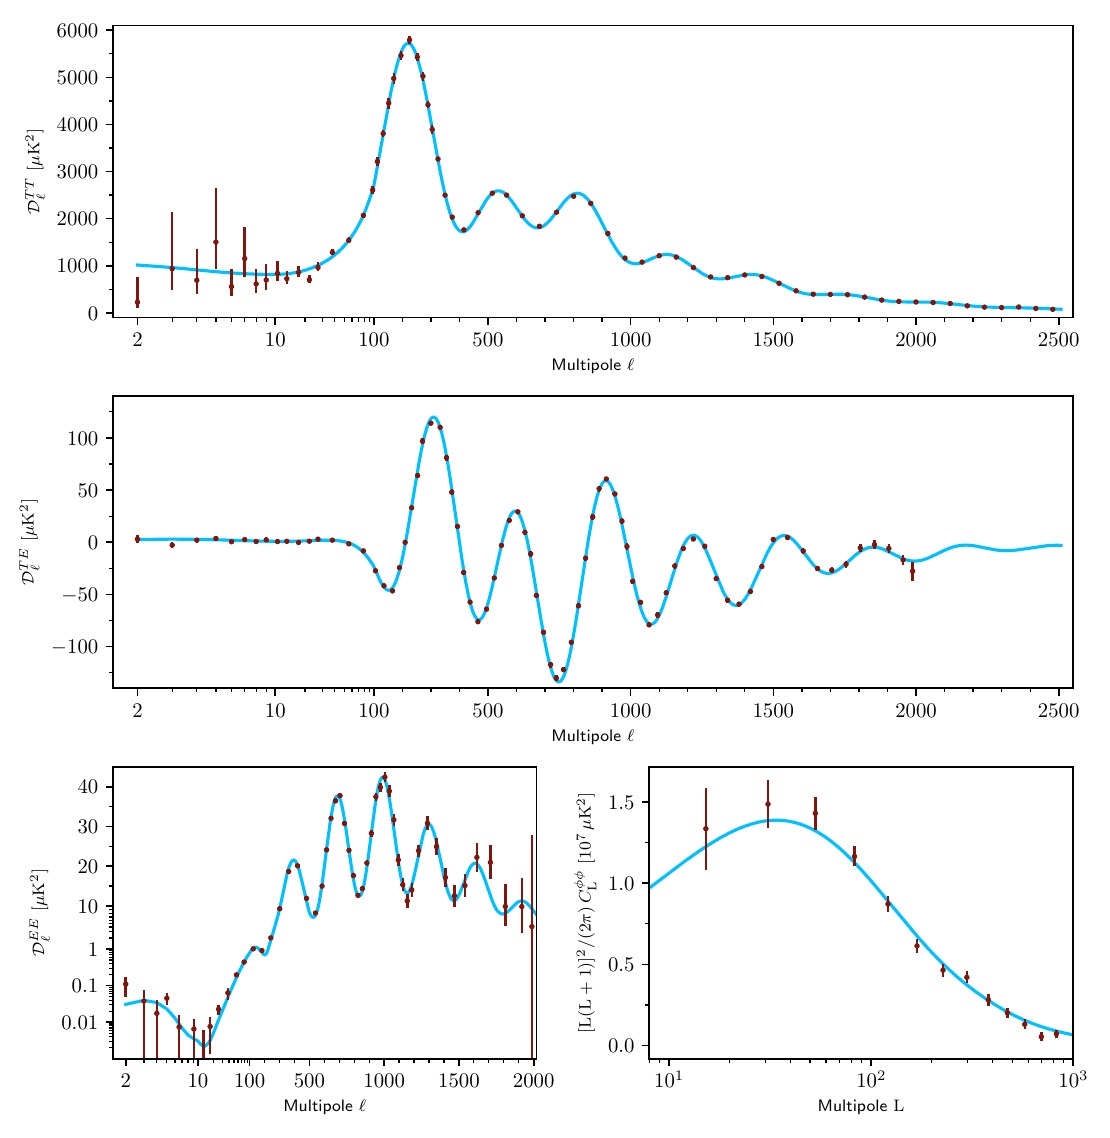
\includegraphics[width=\textwidth]{img/img_04.jpg}
  \caption{\textbf{Planck 2018 CMB angular power spectra.} Foreground-subtracted cross-half-mission power spectra: temperature TT (top left), temperature--polarization cross-spectrum TE (top right), E-mode polarization EE (bottom left), and the gravitational lensing potential (bottom right). Blue lines show the best-fitting $\Lambda$CDM model. The TT spectrum is cosmic-variance limited below $\ell \approx 1800$; the lensing detection exceeds $40\,\sigma$. Acoustic peaks directly constrain the baryon density, dark matter density, and geometry of the Universe. \textit{Reproduced from Planck Collaboration (2020) (Fig.~23), CC-BY 4.0, \copyright\ ESA/Planck Collaboration.}}
  \label{fig:planck_spectra}
\end{figure}

% ──────────────────────────────────────────────────────────────
\section{The Simons Observatory}
\label{sec:so}

The Simons Observatory (SO) is a cosmic microwave background (CMB) survey experiment located in the Atacama Desert in Chile at an elevation of 5200 meters, consisting of an array of three 0.42-meter small aperture telescopes (SATs) and one 6-meter large aperture telescope (LAT). SO will make accurate measurements of the CMB temperature and polarization spanning six frequency bands ranging from 27 to 285 GHz, fielding a total of 60,000 detectors covering angular scales between one arcminute to tens of degrees \cite{Ade2019}.

A central observational challenge is separating the cosmological CMB signal from astrophysical foreground emission. Fig.~\ref{fig:foregrounds} shows the frequency spectra of the dominant components measured by Planck. To address this, we have low frequency (LF, 30/40 GHz), mid frequency (MF, 90/150 GHz), and ultra-high frequency (UHF, 220/285 GHz) designed to understand synchrotron emission, the CMB, and thermal dust emission respectively. The SATs are tailored to search for primordial gravitational waves, with the primary science goal of measuring the primordial tensor-to-scalar ratio $r$ at a target level of $\sigma(r) \approx 0.003$. Currently, two MF SATs and one UHF SAT are actively observing. The UHF SAT is imperative to constraining $r$ --- thermal dust emission has been a leading systematic in this field! The LAT addresses the rest of the science cases listed below, and currently observes at all 6 bands.

\begin{figure}[htbp]
  \centering
  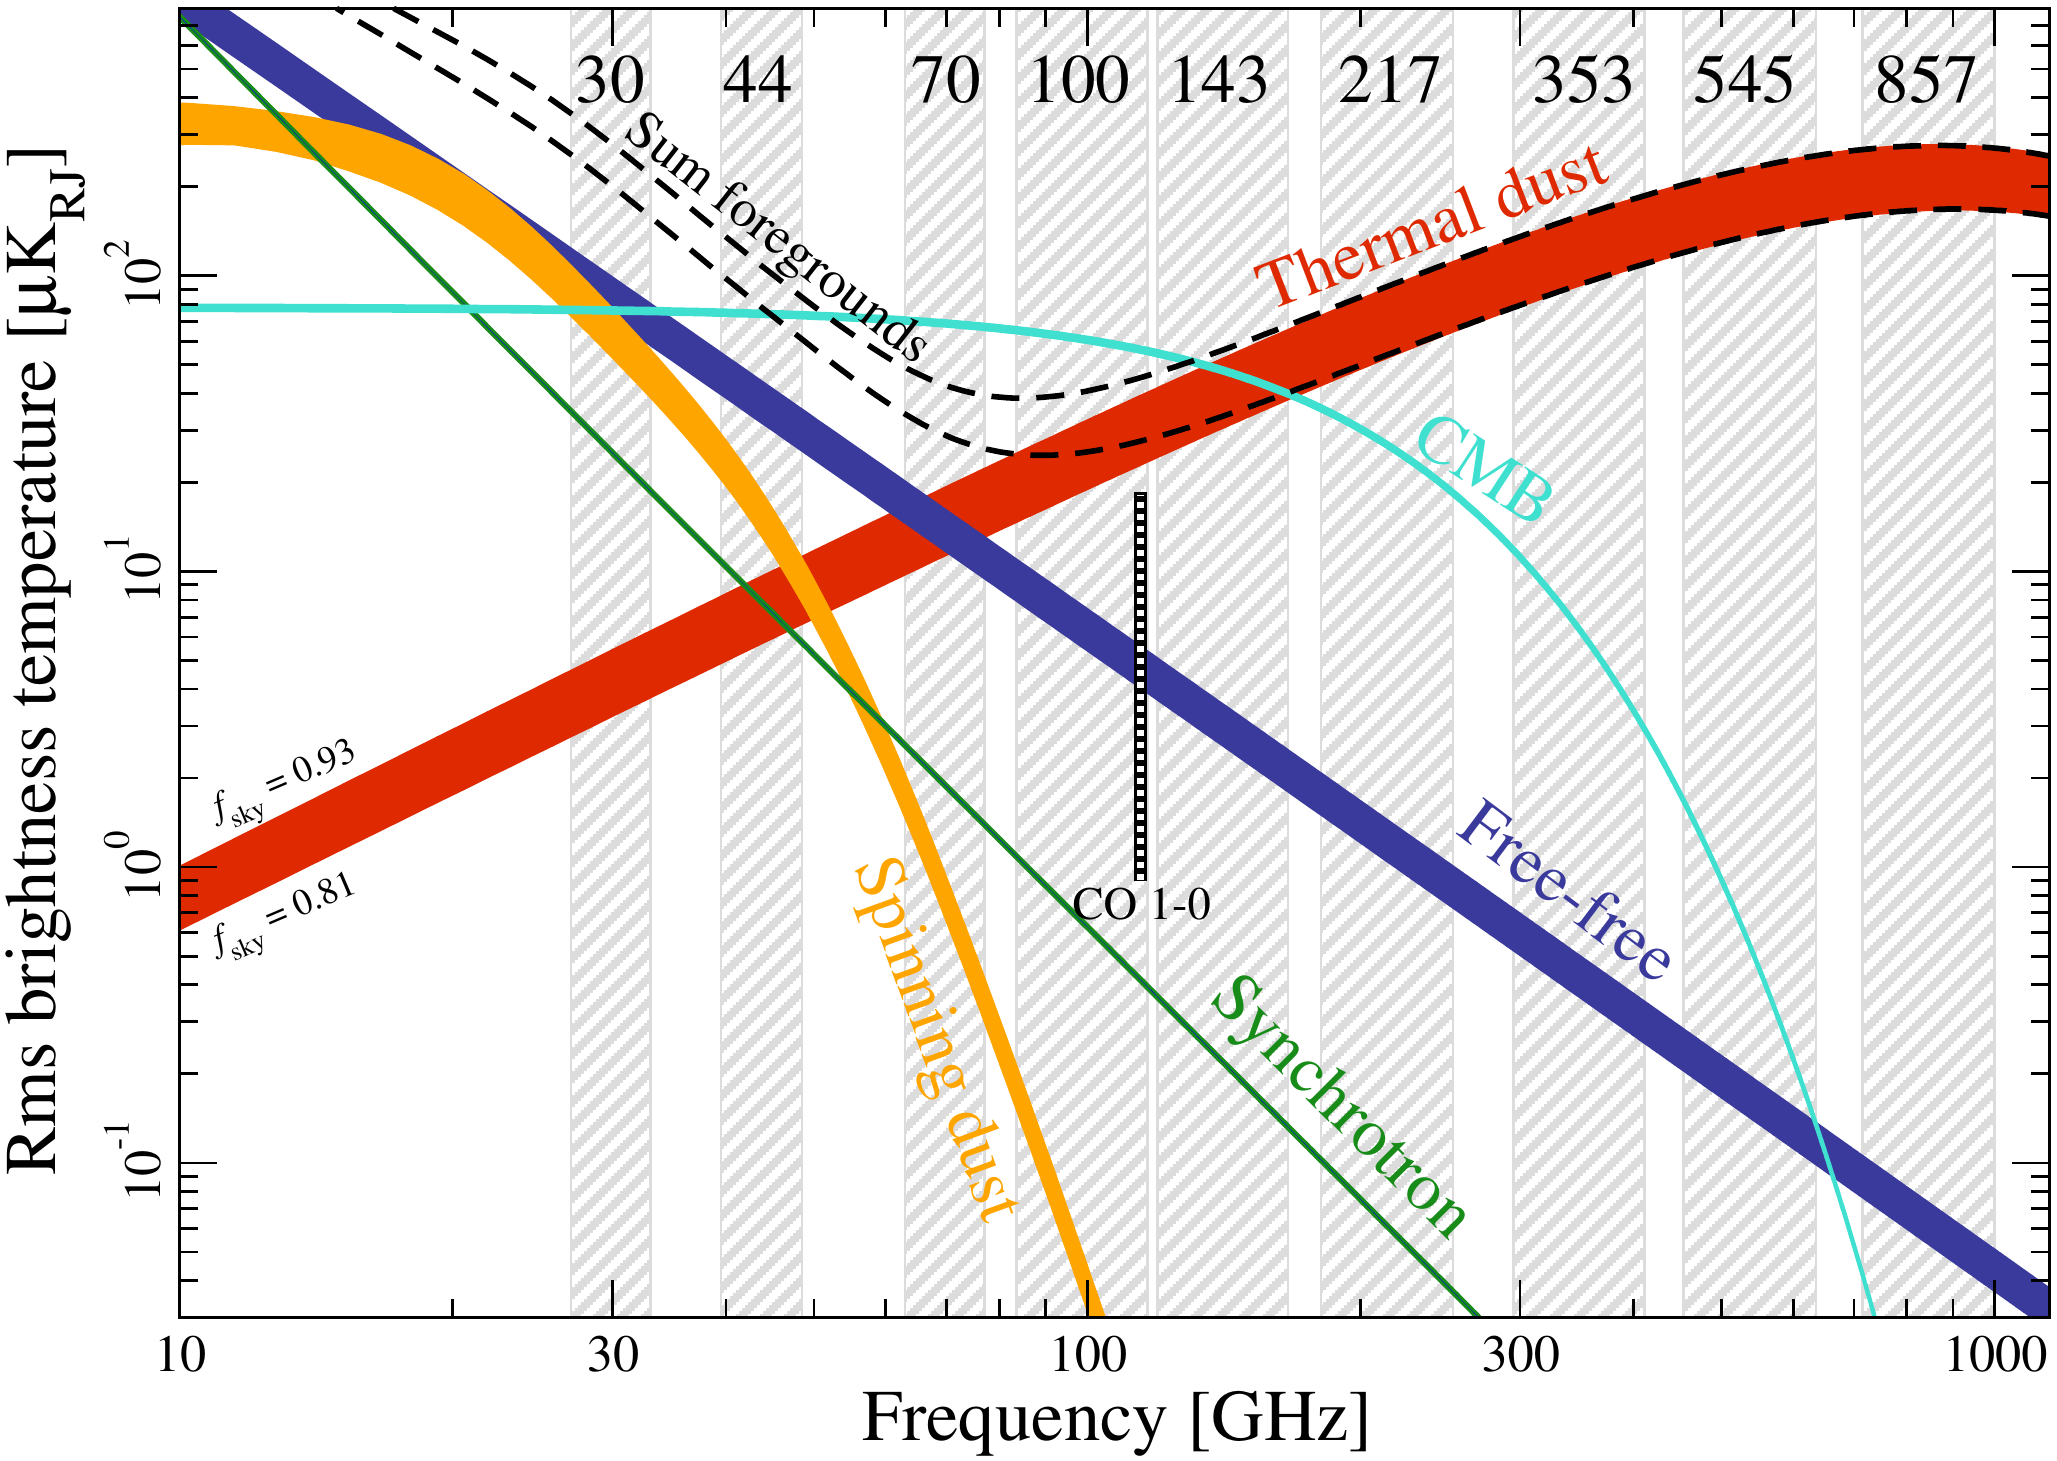
\includegraphics[width=0.48\textwidth]{img/img_05.png}
  \hfill
  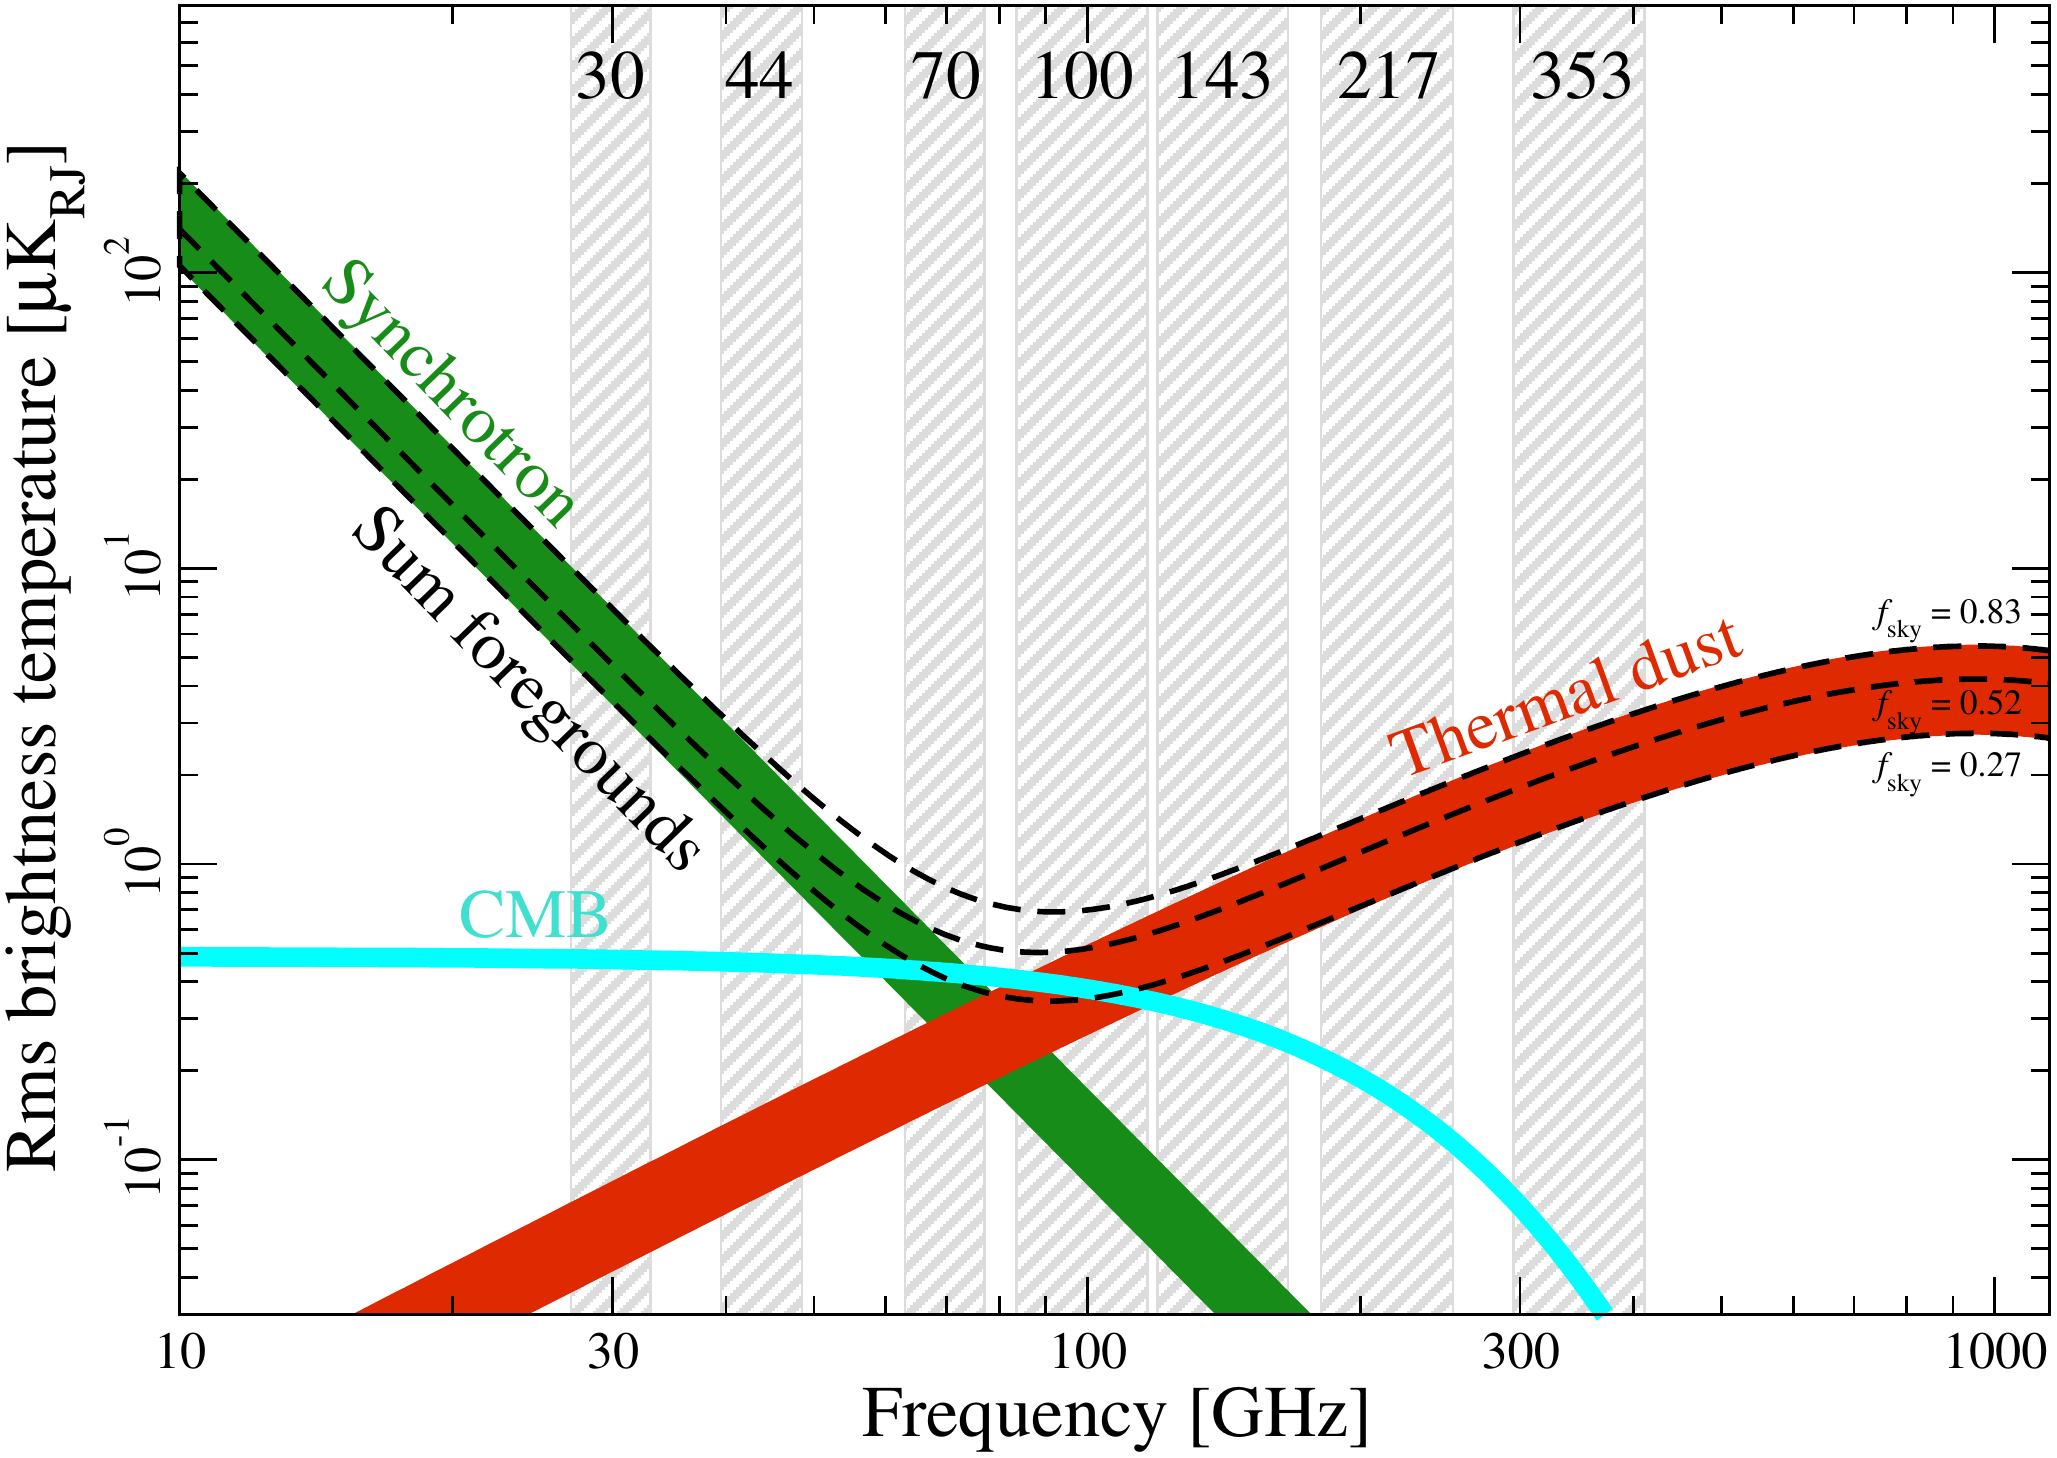
\includegraphics[width=0.48\textwidth]{img/img_06.png}
  \caption{\textbf{Frequency dependence of foreground emission (Planck 2018).} Foreground rms in temperature (left) and polarization (right) vs.\ frequency. In temperature, the CMB dominates near 70--100 GHz, with synchrotron falling steeply at lower frequencies and thermal dust rising above $\sim$100 GHz. Grey vertical bands mark Planck channels; colored bands show the major components. The Simons Observatory's six bands (27--280 GHz) were designed specifically to span this minimum and both foreground regimes. \textit{Reproduced from Planck Collaboration 2020a (Fig.~24), CC-BY 4.0, \copyright\ ESA/Planck Collaboration.}}
  \label{fig:foregrounds}
\end{figure}

\noindent\textbf{Key instrument note:} The \textbf{SAT} (Small Aperture Telescope, 0.5\,m) is optimized for large angular scales ($\ell < 300$) and B-mode polarization --- primarily inflation science. The \textbf{LAT} (Large Aperture Telescope, 6\,m, underilluminated to 5.5\,m) reaches arcminute resolution for all other science cases. Both share 6 frequency bands: 27, 39, 93, 145, 225, 280 GHz.

\subsection*{Key Science Goals \cite{Ade2019}}

\begin{itemize}
  \item \textbf{Inflation:} $\sigma(r) = 0.003$ via B-mode polarization from the SATs.
  \item \textbf{Light relics and neutrinos:} $\sigma(N_\mathrm{eff}) \approx 0.05$ from the CMB damping tail; tighter $\sum m_\nu$ bounds in combination with BAO.
  \item \textbf{Dark energy and lensing:} CMB lensing power spectrum and SZ cluster catalog ($\sim$16,000 clusters) for precision tests of structure growth.
  \item \textbf{Reionization:} kinematic SZ and optical depth measurements.
\end{itemize}

% ──────────────────────────────────────────────────────────────
\section{My Research}
\label{sec:research}

I have designed, integrated, tested, deployed, and commissioned instruments. In particular, I have led the ultra-high frequency small aperture telescope efforts --- this is the first low-$\ell$ 220/280\,GHz telescope to successfully take measurements on the Chilean plateau. Currently, I am making sure that this (along with other) telescopes in SO are operating successfully, making maps with the UHF SAT, calibrating the UHF SAT with planet observations, and analyzing our data for thermal dust emission to help us recover the best constraint on primordial gravitational waves possible with our instruments.

% [LIST RESEARCH PUBS FROM ME OR SO.]

\begin{figure}[htbp]
  \centering
  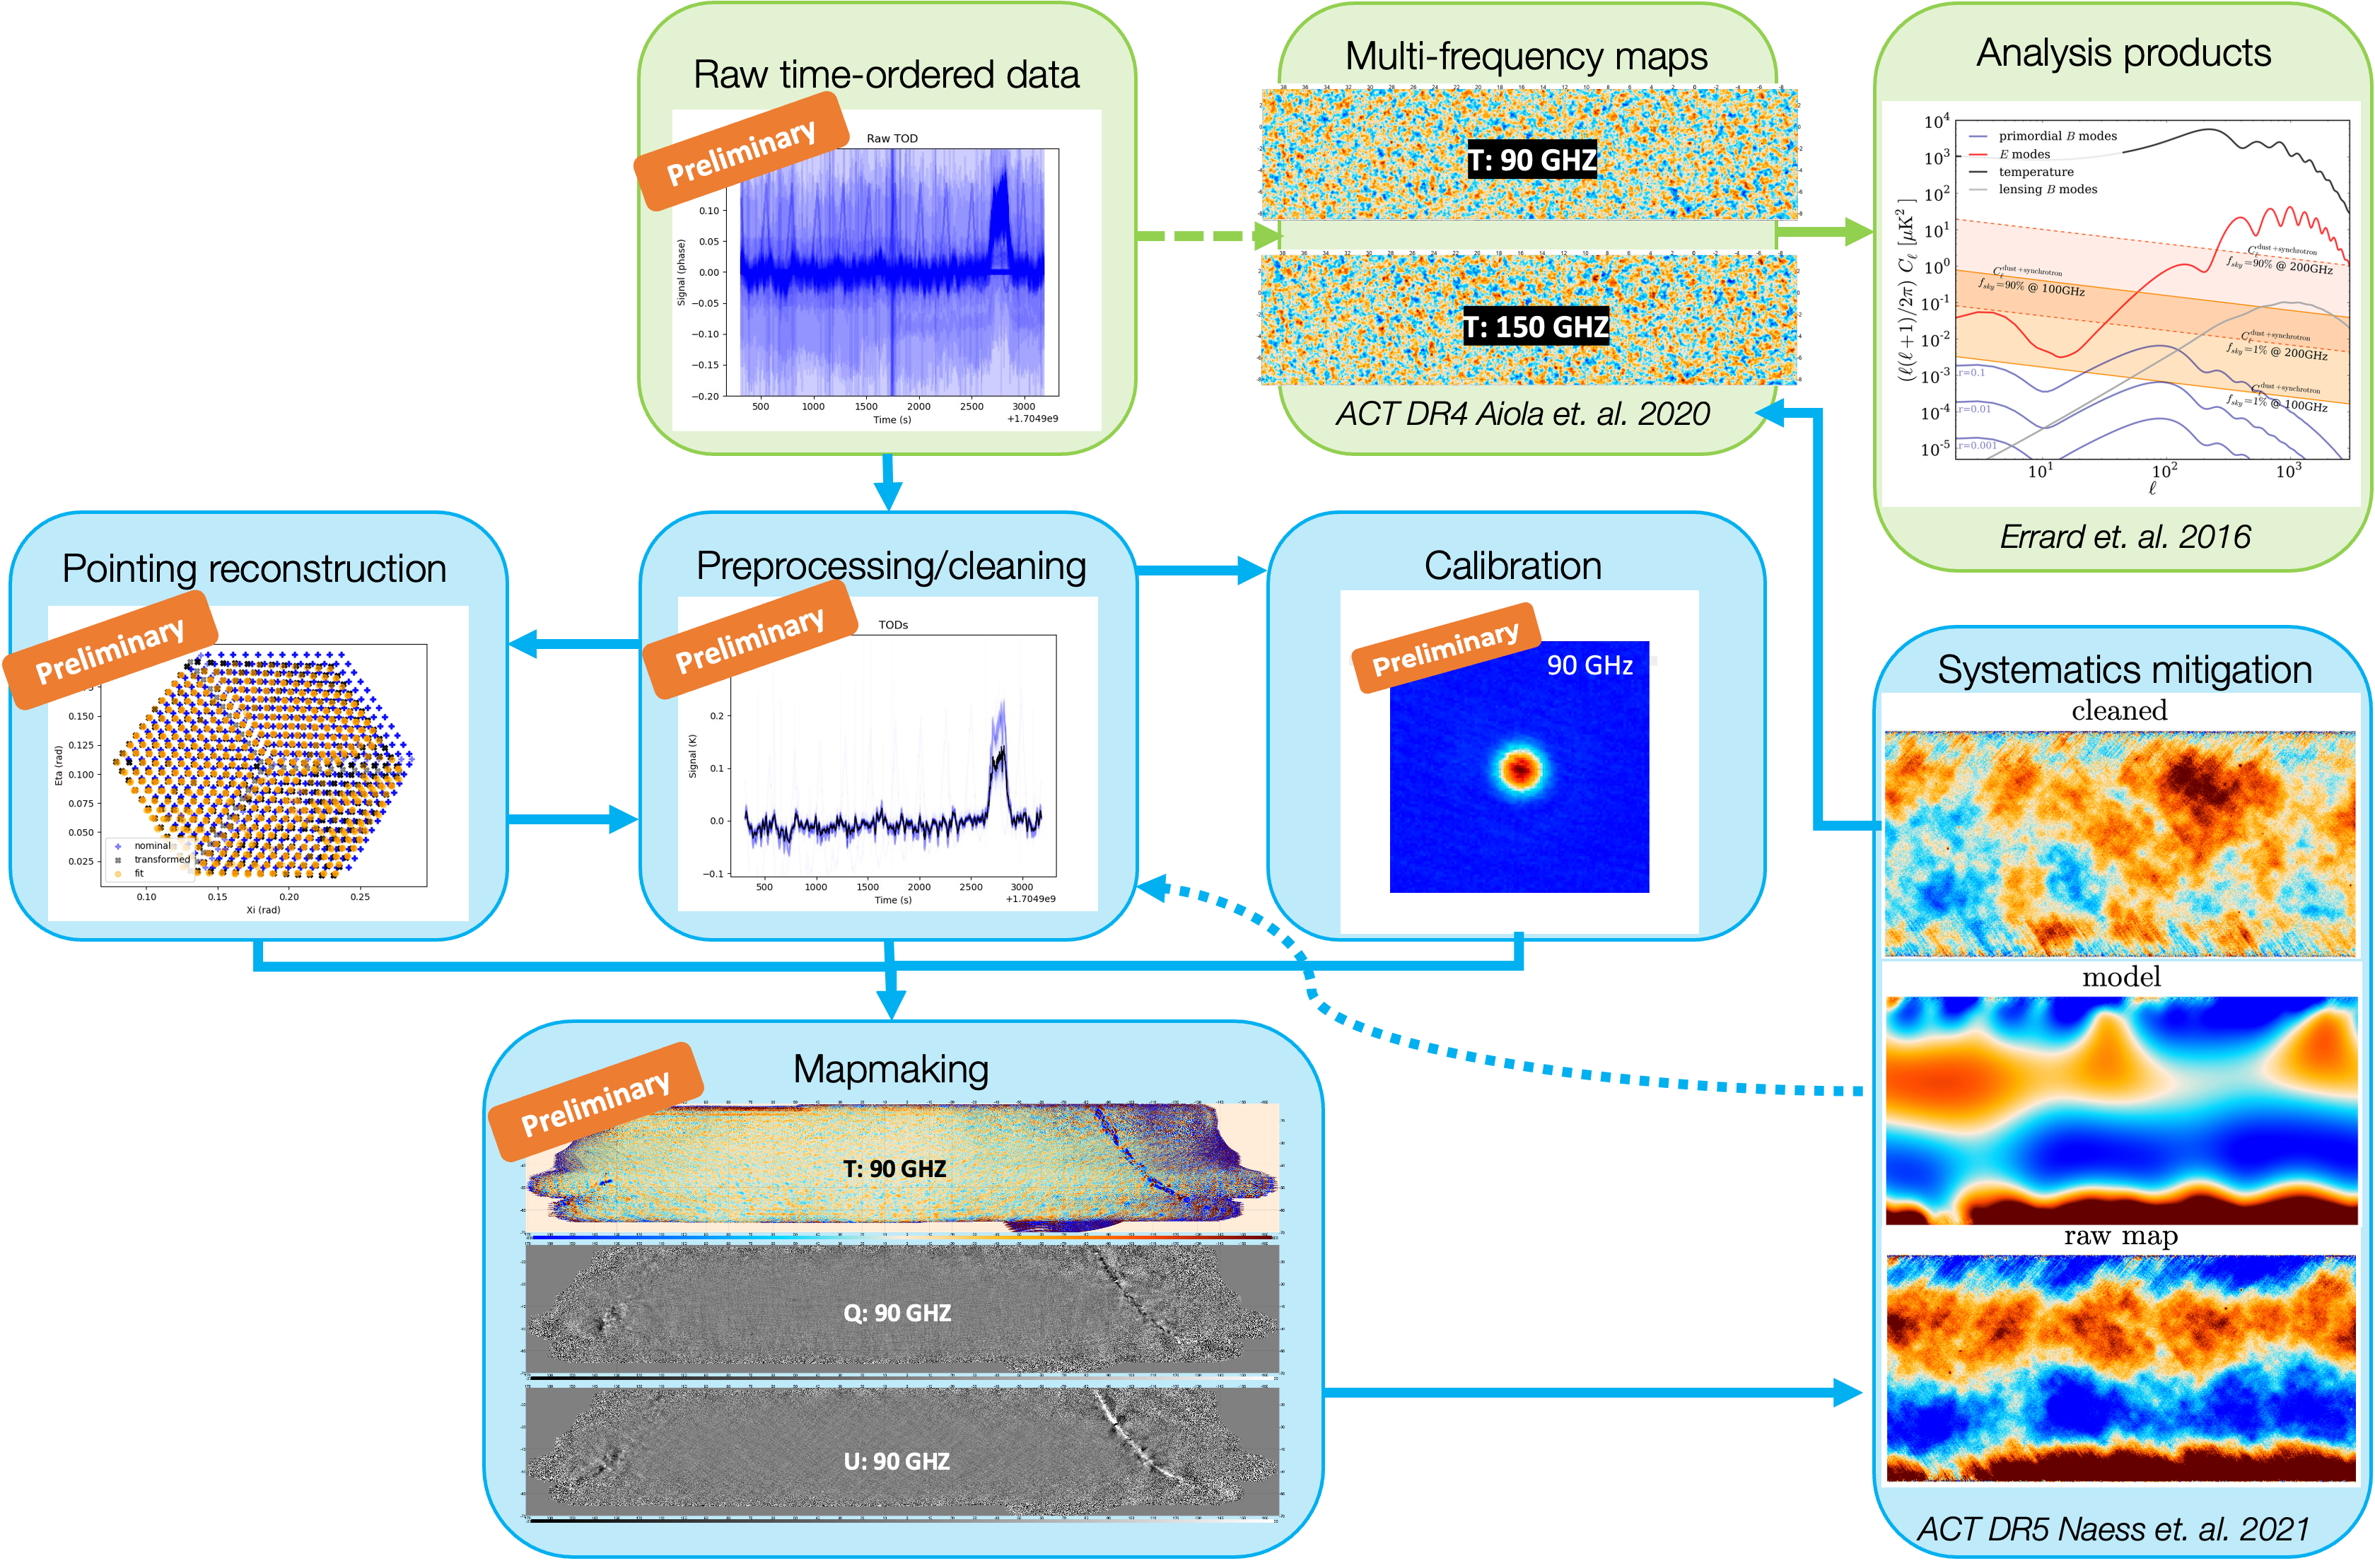
\includegraphics[width=\textwidth]{img/pipeline.png}
  \caption{SO pipeline from raw TODs to maps to analysis products. All images marked `Preliminary' are from real SO data. Other images were taken from older CMB experiments because the SO data is not available to the public yet. Raw TOD example is shown with no processing. From there we process and clean the data, removing e.g.\ bad detectors, jumps, glitches, etc. The cleaned TOD is used to fit for pointing reconstruction so that we know how every detector in our focal plane modules (the hexagon in the image) maps on the sky. This is re-inputted back into the cleaning, and is used to look at calibration sources such as Jupiter (shown). The pointing, preprocessing, and calibration are all used to make maps (T is temperature and Q, U are linear polarization Stokes parameters). Then from there we can do systematics testing and removal. Shown is the effect of ground pick-up removal from ACT DR5 \cite{Naess2021}. Cleaned multi-frequency maps are then released (ACT DR4 image from \cite{Aiola2020}), and can be used for final analysis products and cosmological constraints (power spectrum image from \cite{Errard2016}).}
  \label{fig:pipeline}
\end{figure}

% ──────────────────────────────────────────────────────────────
\section*{References}
\label{sec:refs}

\begin{thebibliography}{99}

\bibitem{Ade2019}
  Ade, P., et al.\ (SO Collaboration) 2019, ``The Simons Observatory: Science Goals and Forecasts,'' \textit{JCAP}, 2019, 056.
  \url{https://doi.org/10.1088/1475-7516/2019/02/056}

\bibitem{CMBHD2022}
  CMB-HD Collaboration (Aiola, S., et al.) 2022, ``Snowmass2021 CMB-HD White Paper,'' arXiv:2203.05728.
  \url{https://arxiv.org/abs/2203.05728} (CC-BY 4.0)

\bibitem{Madhavacheril2023}
  Madhavacheril, M.\,S., et al.\ 2023, ``The Atacama Cosmology Telescope: High-Resolution Component-Separated Maps Across One-Third of the Sky,'' \textit{ApJ}, 962, 113.
  \url{https://doi.org/10.3847/1538-4357/acff5f} (CC-BY 4.0)

\bibitem{Planck2020a}
  Planck Collaboration 2020a, ``Planck 2018 results. I. Overview and the cosmological legacy of Planck,'' \textit{A\&A}, 641, A1.
  \url{https://doi.org/10.1051/0004-6361/201833880} (CC-BY 4.0)

\bibitem{Planck2020b}
  Planck Collaboration 2020b, ``Planck 2018 results. VI. Cosmological parameters,'' \textit{A\&A}, 641, A6.
  \url{https://doi.org/10.1051/0004-6361/201833910} (CC-BY 4.0)

\bibitem{Aiola2020}
  Aiola, S., et al.\ (ACT Collaboration) 2020, ``The Atacama Cosmology Telescope: DR4 Maps and Cosmological Parameters,'' \textit{JCAP}, 2020, 047.
  \url{https://doi.org/10.1088/1475-7516/2020/12/047}

\bibitem{Naess2021}
  Naess, S., et al.\ (ACT Collaboration) 2021, ``The Atacama Cosmology Telescope: A Beam and Calibration Analysis for the 2017--2018 CMB Data,'' \textit{JCAP}, 2021, 044.
  \url{https://doi.org/10.1088/1475-7516/2021/10/044}

\bibitem{Errard2016}
  Errard, J., et al.\ 2016, ``Robust forecasts on fundamental physics from the foreground-obscured, gravitationally-lensed CMB polarization,'' \textit{JCAP}, 2016, 052.
  \url{https://doi.org/10.1088/1475-7516/2016/03/052}

\end{thebibliography}

\end{document}
